\documentclass[10pt,landscape]{article}
\usepackage{multicol}
\usepackage{calc}
\usepackage{ifthen}
\usepackage[landscape]{geometry}
\usepackage{amsmath,amsthm,amsfonts,amssymb}
\usepackage{color,graphicx}
\usepackage{hyperref}
\usepackage[font=scriptsize,labelfont=bf]{caption}
\usepackage{wrapfig}
\usepackage{graphicx,calc}
%\usepackage{pbox}

\pdfinfo{
  /Title (Leistungelektronik)
  /Creator (TeX)
  /Producer (pdfTeX 1.40.0)
  /Author (Noah Huetter)
  /Subject (Leistungelektronik)
  /Keywords (Leistungelektronik,ETH)}

% This sets page margins to .5 inch if using letter paper, and to 1cm
% if using A4 paper. (This probably isn't strictly necessary.)
% If using another size paper, use default 1cm margins.
\ifthenelse{\lengthtest { \paperwidth = 11in}}
    { \geometry{top=.5in,left=.5in,right=.5in,bottom=.5in} }
    {\ifthenelse{ \lengthtest{ \paperwidth = 297mm}}
        {\geometry{top=1cm,left=1cm,right=1cm,bottom=1cm} }
        {\geometry{top=1cm,left=1cm,right=1cm,bottom=1cm} }
    }

% Turn on simple page number
\pagestyle{plain}

% Redefine section commands to use less space
\makeatletter
\renewcommand{\section}{\@startsection{section}{1}{0mm}%
                                {-1ex plus -.5ex minus -.2ex}%
                                {0.5ex plus .2ex}%x
                                {\normalfont\large\bfseries}}
\renewcommand{\subsection}{\@startsection{subsection}{2}{0mm}%
                                {-1explus -.5ex minus -.2ex}%
                                {0.5ex plus .2ex}%
                                {\normalfont\normalsize\bfseries}}
\renewcommand{\subsubsection}{\@startsection{subsubsection}{3}{0mm}%
                                {-1ex plus -.5ex minus -.2ex}%
                                {1ex plus .2ex}%
                                {\normalfont\small\bfseries}}
\makeatother

% Define BibTeX command
\def\BibTeX{{\rm B\kern-.05em{\sc i\kern-.025em b}\kern-.08em
    T\kern-.1667em\lower.7ex\hbox{E}\kern-.125emX}}

% Don't print section numbers
\setcounter{secnumdepth}{0}


\setlength{\parindent}{0pt}
\setlength{\parskip}{1pt plus 0.5ex}

%My Environments
\newtheorem{example}[section]{Example}
% -----------------------------------------------------------------------
\newcommand{\eqn}[3]
{
  \begin{minipage}[#1]{#2}
    \[ #3 \]
  \end{minipage}
}
\newcommand{\feqn}[3]
{
\fbox{
  \begin{minipage}[#1]{#2}
    \[ #3 \]
  \end{minipage}
}
}
 

 
\begin{document}
\raggedright
\footnotesize
\begin{multicols}{2}



% multicol parameters
% These lengths are set only within the two main columns
%\setlength{\columnseprule}{0.25pt}
\setlength{\premulticols}{1pt}
\setlength{\postmulticols}{1pt}
\setlength{\multicolsep}{1pt}
\setlength{\columnsep}{2pt}

\begin{center}
     \Large{\underline{Leistungelektronik}} \\
\end{center}
% -----------------------------------------------------------------------
\IfFileExists{build/revision.tex}{
  \input{build/revision.tex}
  Author: Noah Huetter \hfill Date: \compiledate \hspace{1em} Commit: \revision
}{Author: Noah Huetter}


% -----------------------------------------------------------------------
\vspace{2mm}\hrule
\section{Allgemein}
\eqn{h}{0.23\linewidth}{ i_L(t) = \frac{1}{L}\int u_L(t)dt }
\eqn{h}{0.23\linewidth}{ u_L(t) = L\frac{di_L(t)}{dt} }

% -----------------------------------------------------------------------
\vspace{2mm}\hrule
\section{Tiefsetzsteller}

\begin{center}
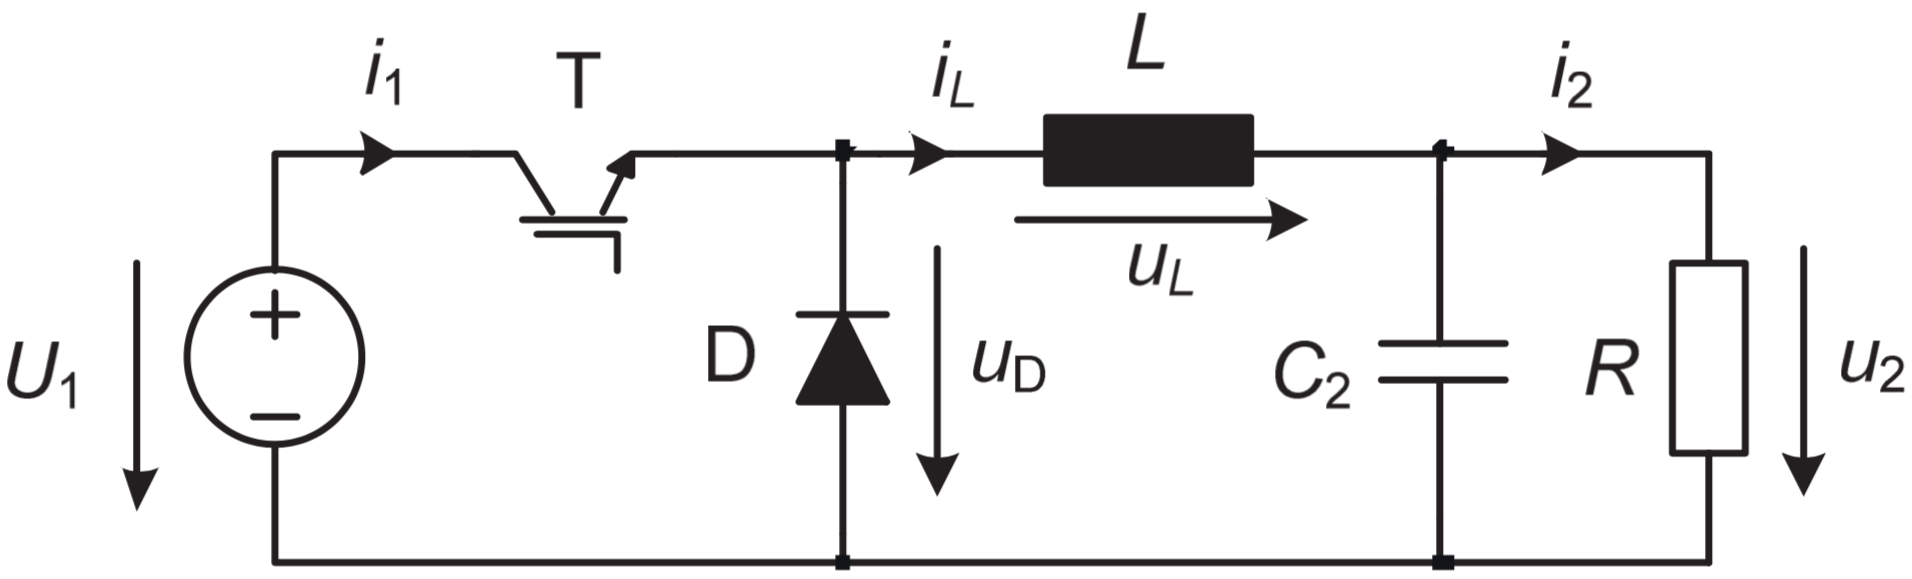
\includegraphics[width=0.8\linewidth]{img/sch_buck.png}%
\captionof{figure}{Tiefsetzsteller}%
\end{center}

\subsection{Kontinuierlicher Stromfluss}
\eqn{h}{0.25\linewidth}{ D3 = \frac{I_1}{I_2} = \frac{U_2}{U_1} }
\eqn{h}{0.25\linewidth}{ \Delta i_{Lpp} = \frac{U_2}{L}(1-D)T_S}
\eqn{h}{0.25\linewidth}{ \Delta u_{2pp}=\Delta U_C = \frac{U_2}{L}(1-D) T_S \frac{T_S}{8 \cdot C}}

\subsection{Diskontinuierlicher Stromfluss}
\eqn{h}{0.4\linewidth}{ I_{2g} = \frac{1}{2} \Delta i_{Lpp} = \frac{U_2}{2 \cdot L}(1-D)T_S}
\eqn{h}{0.25\linewidth}{ R_{g} = \frac{2L}{(1-D) \cdot T_S}}
\eqn{h}{0.25\linewidth}{ U_2=U_1 \frac{D_1}{D_1+D_2} }
\eqn{h}{0.3\linewidth}{ I_{2g,max}=I_{2g}|_{D=0.5} = \frac{U_1 T_S}{8L} }
\eqn{h}{0.3\linewidth}{ \frac{U_2}{U_1}=\frac{D^2}{D^2+\frac{1}{4} \frac{I_2}{I_{2g,max}} } }
\eqn{h}{0.25\linewidth}{ D = \frac{1}{2} \sqrt{\frac{I_2/I_{2g,max}}{U_1/U_2-1}} }

% -----------------------------------------------------------------------
\vspace{2mm}\hrule
\section{Hochsetzsteller}

\begin{center}
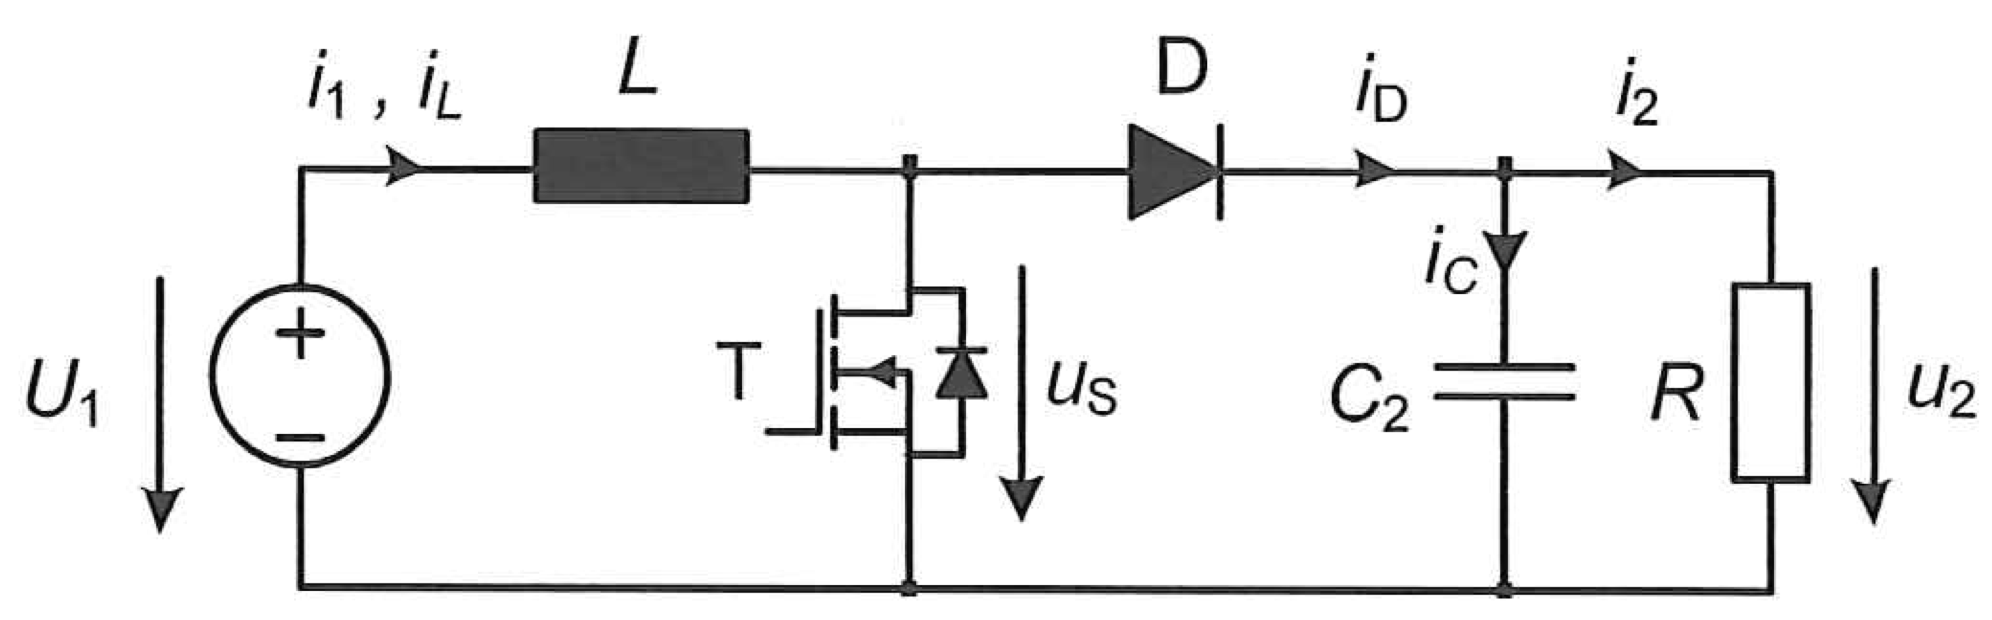
\includegraphics[width=0.8\linewidth]{img/sch_boost.png}%
\captionof{figure}{Hochsetzsteller}%
\end{center}

\subsection{Kontinuierlicher Stromfluss}
\eqn{h}{0.23\linewidth}{ D = 1 - \frac{U_1}{U_2} }
\eqn{h}{0.23\linewidth}{ \frac{I_2}{I_1}=1-D }
\eqn{h}{0.23\linewidth}{ \Delta U_{2pp} = \frac{U_2}{R}\frac{DT_s}{C_2} }

\subsection{Diskontinuierlicher Stromfluss}
\eqn{h}{0.3\linewidth}{ I_{Lg} = \frac{1}{2} \frac{(U_2-U_1)}{L}(1-D)T_s }
\eqn{h}{0.3\linewidth}{ I_{1g} = \frac{1}{2} \frac{U_2}{L}D(1-D)T_s }
\eqn{h}{0.3\linewidth}{ I_{2g,max} = I_{2g}|_{D=1/3} = \frac{2}{27}\frac{U_2}{L}T_S }

\eqn{h}{0.3\linewidth}{ D= \sqrt{\frac{4}{27}\frac{U_2}{U_1} \left (\frac{U_2}{U_1}-1 \right ) \frac{I_2}{I_{2g,max}} } }

% \eqn{h}{0.25\linewidth}{ }
% -----------------------------------------------------------------------
\vspace{2mm}\hrule
\section{Tief-Hochsetzsteller}

\begin{center}
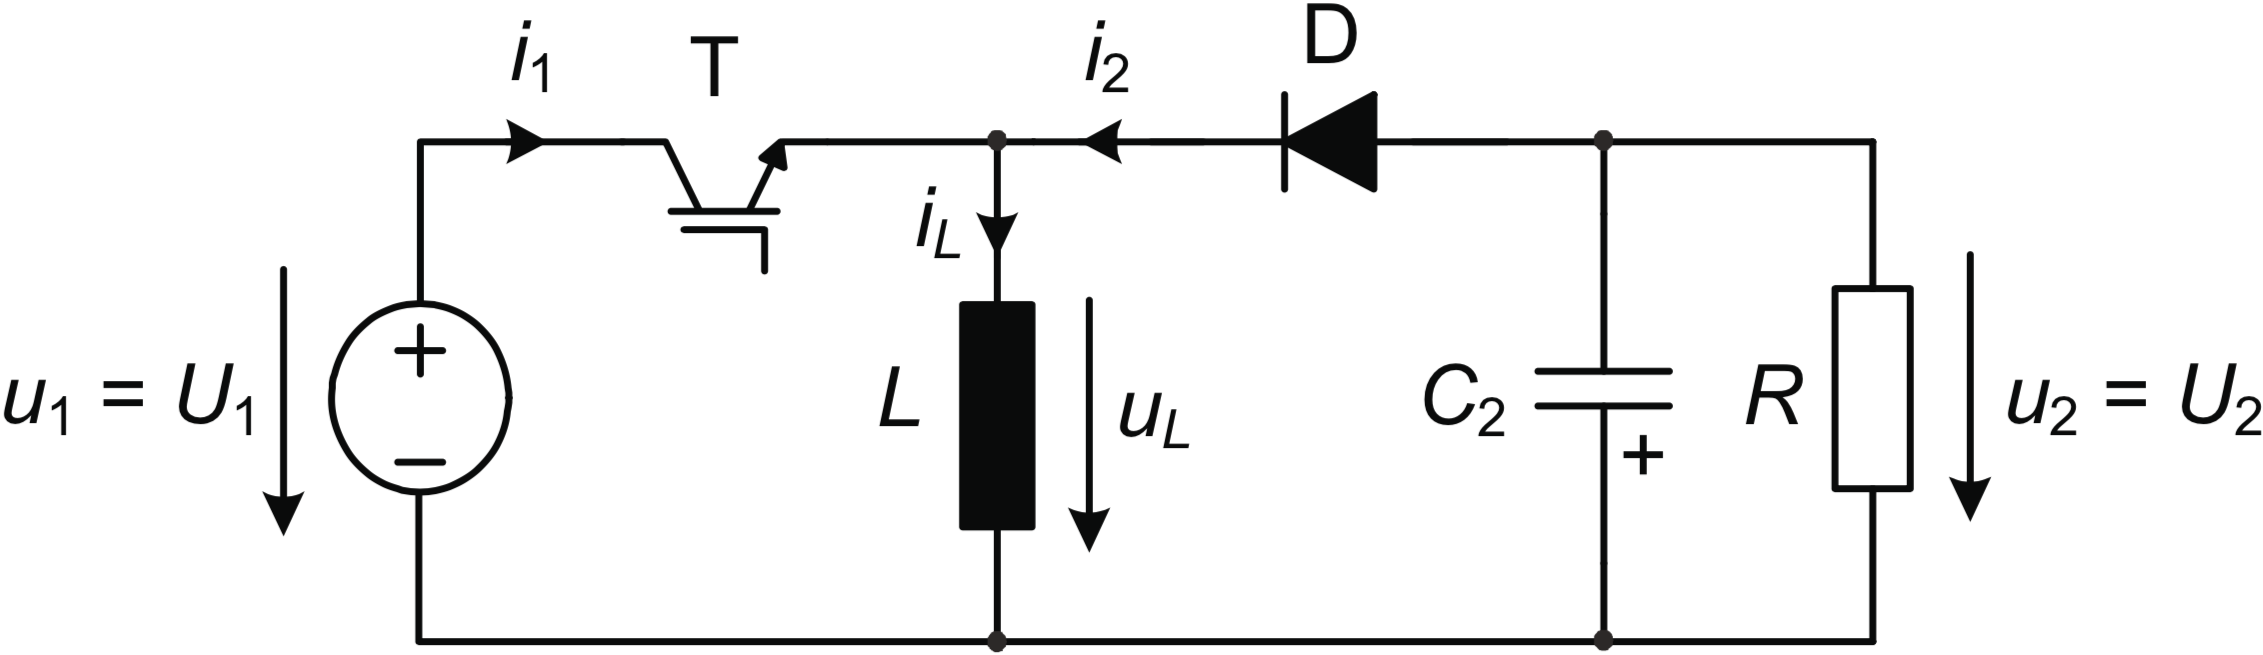
\includegraphics[width=0.8\linewidth]{img/sch_invers.png}%
\captionof{figure}{Tief-Hochsetzsteller}%
\end{center}

\subsection{Kontinuierlicher Stromfluss}
\eqn{h}{0.23\linewidth}{ \frac{U_2}{U_1} = -\frac{D}{1-D} }
\eqn{h}{0.23\linewidth}{ \frac{I_2}{I_1}=\frac{1-D}{D} }

\subsection{Diskontinuierlicher Stromfluss}
\eqn{h}{0.3\linewidth}{ I_{Lg} = \frac{1}{2} \frac{-U_2}{L}(1-D)T_s }
\eqn{h}{0.3\linewidth}{ I_{2g} = \frac{1}{2} \frac{-U_2}{L}(1-D)^2T_s }
\eqn{h}{0.3\linewidth}{ I_{2g,max} = -\frac{1}{2} \frac{U_2}{L}T_s }

\eqn{h}{0.3\linewidth}{ D = -\frac{U_2}{U_1} \sqrt{\frac{I_2}{I_{2g,max}}} }


% -----------------------------------------------------------------------
\vspace{2mm}\hrule
\section{PFC Einphasen Gleichrichter}

\begin{center}
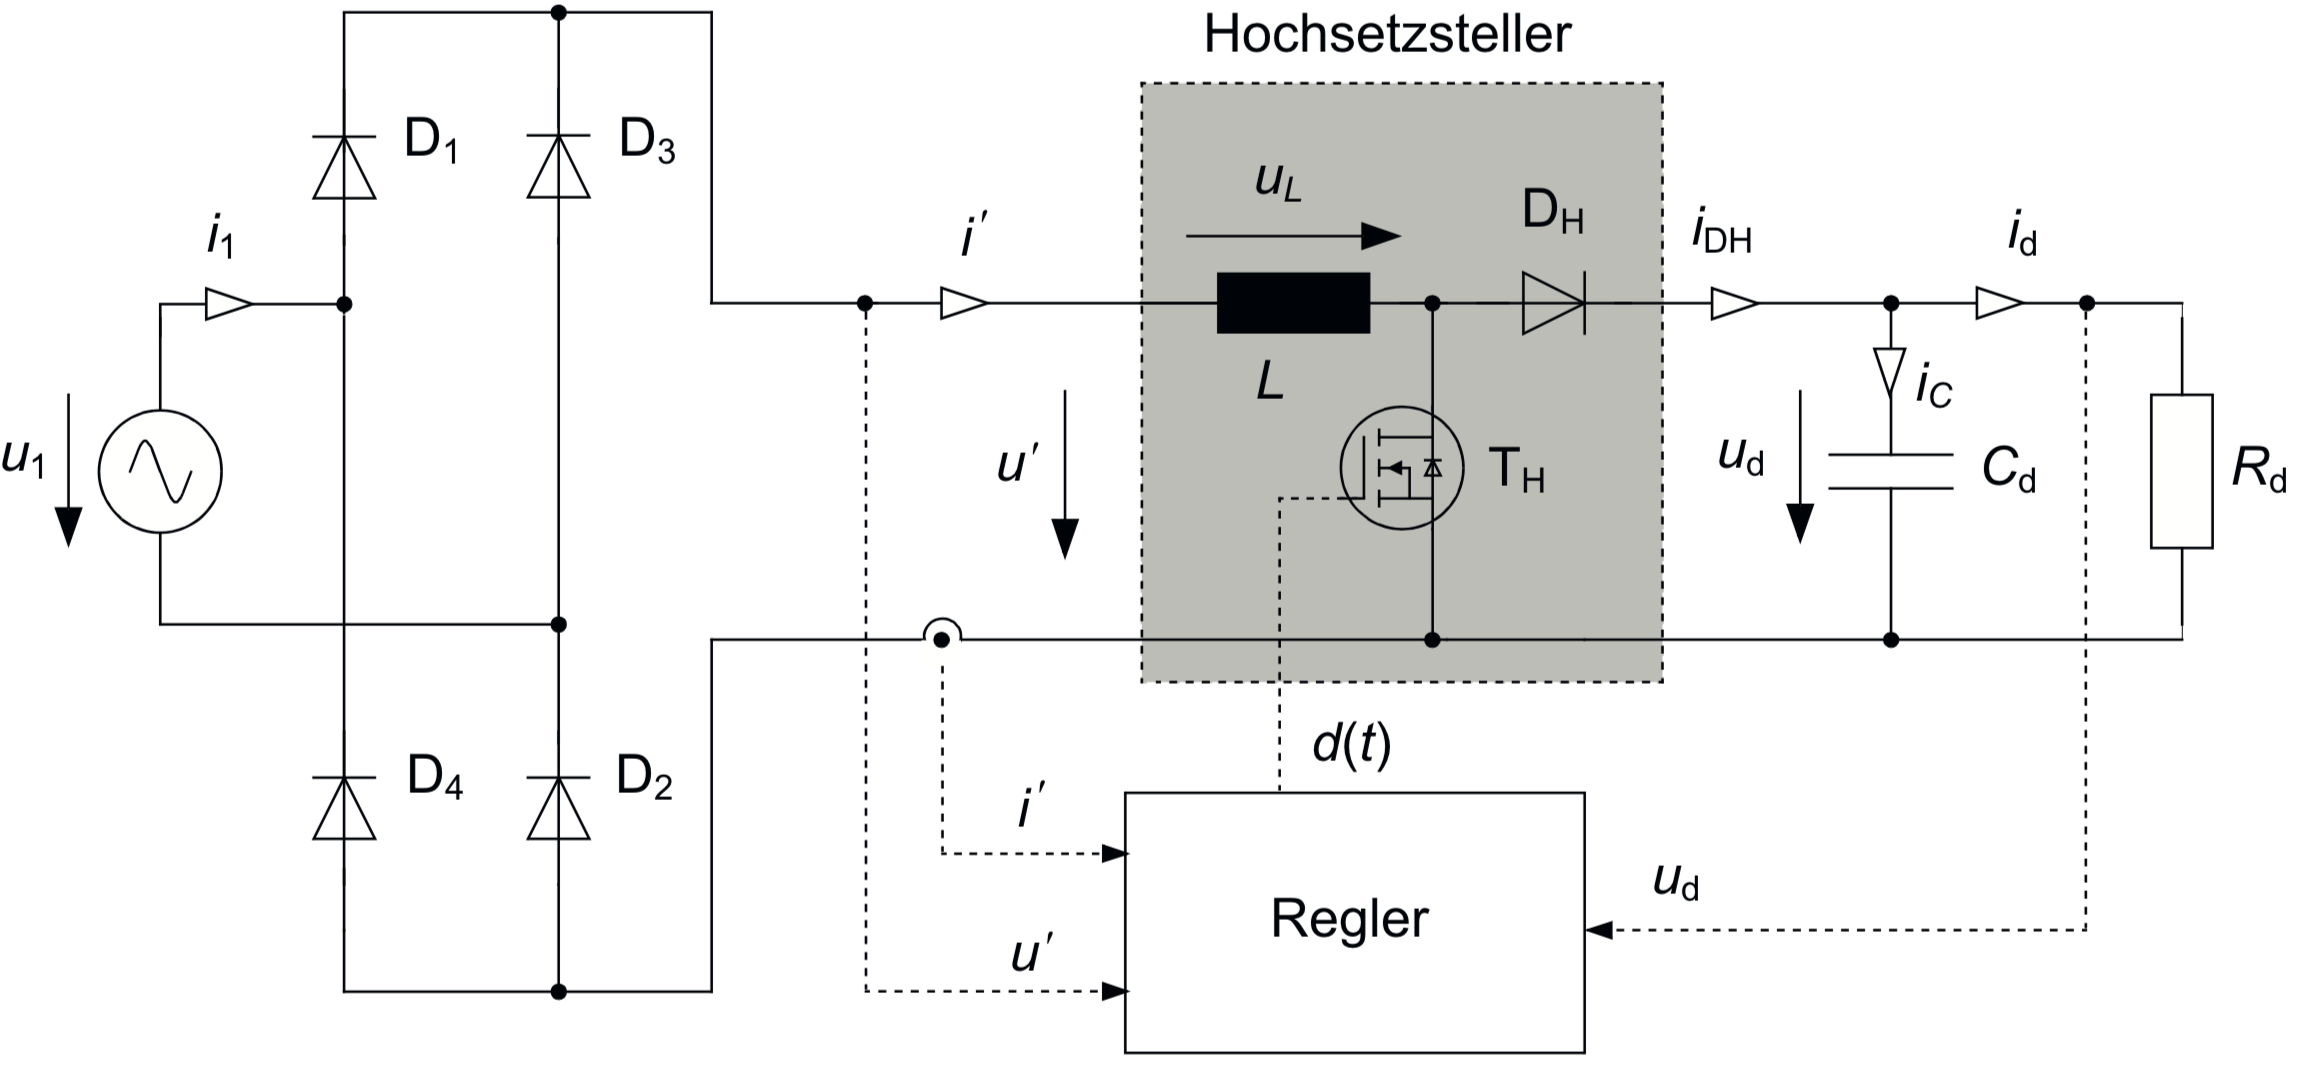
\includegraphics[width=0.8\linewidth]{img/sch_pfc.png}%
\captionof{figure}{PFC Einphasen Gleichrichter}%
\end{center}

\subsection{Toleranzbandregelung}
\eqn{h}{0.23\linewidth}{ i'_{max}=(1+k)i'^* }
\eqn{h}{0.23\linewidth}{ i'_{min}=(1-k)i'^* }
\eqn{h}{0.23\linewidth}{ \Delta i_{pp} = 2k\cdot \hat{i}'^* |sin(\omega t)| }



% -----------------------------------------------------------------------
\vspace{2mm}\hrule
\section{Netzgeführte Stromrichter}
Text

% -----------------------------------------------------------------------
\vspace{2mm}\hrule
\section{Induktivität Dimensionierung}
Text

% -----------------------------------------------------------------------
\vspace{2mm}\hrule
\section{Trafo Dimensionierung}
Text

% -----------------------------------------------------------------------
\vspace{2mm}\hrule
\section{Sperrwandler}
Text

% -----------------------------------------------------------------------
\vspace{2mm}\hrule
\section{Durchflusswandler}
Text

% -----------------------------------------------------------------------
\vspace{2mm}\hrule
\section{Einphasen Gleichspannungswechselrichter}
Text

% -----------------------------------------------------------------------
\vspace{2mm}\hrule
\section{Dreiphasen Gleichspannungswechselrichter}
Text

\clearpage

% You can even have references
\rule{0.3\linewidth}{0.25pt}
%\scriptsize
%\bibliographystyle{abstract}
%\bibliography{refFile}
\end{multicols}
\end{document}
